\begin{figure}[!htbp]
\centering
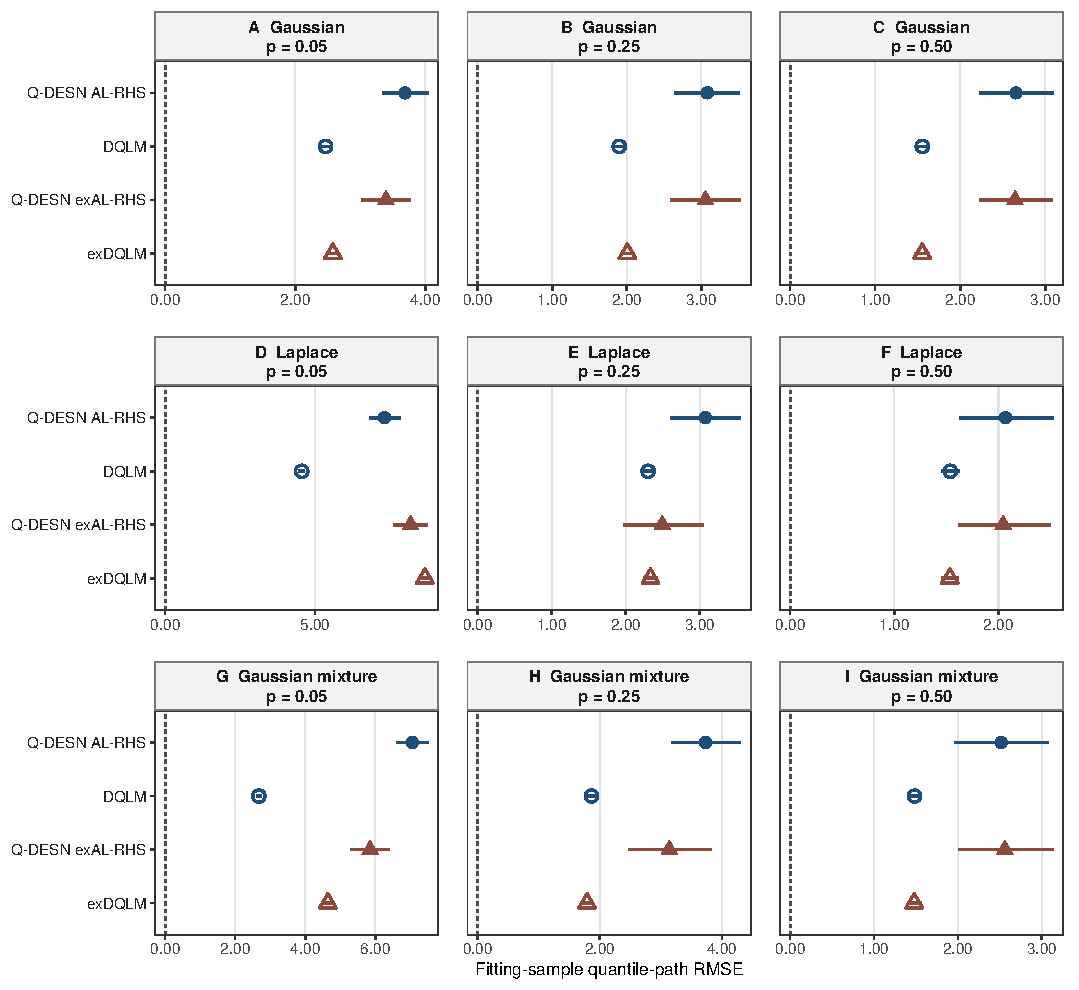
\includegraphics[width=0.98\textwidth]{figures/ch04-qdesn/independent_simulation/qdesn_validation_500obs_v14_vb_fit_rmse_intervals.pdf}
\caption{Variational fitting-sample recovery in the single-quantile
simulation. Points are variational posterior means of quantile-path RMSE and
horizontal segments are equal-tailed approximate 95\% variational posterior
intervals; lower values are better. Navy circles identify the \(\AL\) models
and muted-brick triangles the \(\exAL\) models; filled symbols denote Q--DESN
and open symbols the corresponding dynamic quantile linear model. Panels A--I
identify the data-generating family and probability level and use separate
horizontal scales. The dashed line marks exact recovery of the known
conditional quantile path. Intervals condition on the simulated series,
evaluation design, and case-specific selected specification.}
\figalt{Nine panels compare approximate variational fitting-sample
quantile-path RMSE means and 95 percent intervals for four models across three
innovation families and three probability levels. Lower values are better.}
\label{qdesn:fig:simulation-500obs-vb-fit-rmse-intervals}
\end{figure}
